%!TEX program = pdflatex
%# -*- coding: utf-8 -*-
%!TEX encoding = UTF-8 Unicode

\documentclass[12pt,oneside,a4paper]{article}

%% ------------------------------------------------------
%% load packages
\usepackage{geometry}
\geometry{verbose,tmargin=2cm,bmargin=2cm,lmargin=2cm,rmargin=2cm}
\usepackage[pdfusetitle,
 bookmarks=true,bookmarksnumbered=true,bookmarksopen=true,bookmarksopenlevel=2,
 breaklinks=false,pdfborder={0 0 1},backref=false,colorlinks=false,
 unicode=true]
 {hyperref}
\hypersetup{pdfstartview={XYZ null null 1}}
\usepackage{url}
\setcounter{secnumdepth}{2}
\setcounter{tocdepth}{2}
\usepackage{microtype}

\usepackage{amsmath, amsthm, amssymb, amsfonts}
\usepackage[retainorgcmds]{IEEEtrantools}

% \usepackage{algorithm}
% \usepackage{algorithmic}
% \renewcommand{\algorithmicrequire}{\textbf{Input:}}
% \renewcommand{\algorithmicensure}{\textbf{Output:}}
\usepackage[algoruled, vlined]{algorithm2e}

\usepackage[T1]{fontenc}
\usepackage[utf8]{inputenc}
\usepackage[mono=false]{libertine}
\usepackage[libertine]{newtxmath}
\linespread{1.05}
\setlength{\parskip}{.5\baselineskip}
% \usepackage[toc,eqno,enum,bib,lineno]{tabfigures}

\usepackage{graphics}
\usepackage{graphicx}
\usepackage[figure]{hypcap}
\usepackage[hypcap]{caption}
\usepackage{tikz}
\usepackage{tikz-cd}
%\usepackage{grffile}
%\usepackage{float}
\usepackage{pdfpages}
\usepackage{pdflscape}
\usepackage{needspace}

\usepackage{multirow}
\usepackage{booktabs}
\usepackage{threeparttable}
\usepackage{dcolumn}
\usepackage{tabu}

\usepackage{verbatim}

% \usepackage[square,numbers,super,comma,sort]{natbib}
\usepackage[backend=biber, style=nature, sorting=none, isbn=false, url=false, doi=false]{biblatex}
\addbibresource{ref.bib}
\usepackage[]{authblk}

%% Class, Exam, Date, etc.
\newcommand{\class}{CSCI 5525: Machine Learning}
\newcommand{\term}{Fall 2015}
\newcommand{\examnum}{Homework 2}
\newcommand{\hmwkTitle}{\class \\[1ex] \examnum}
\newcommand{\hmwkAuthorName}{Jingxiang Li}

\title{\hmwkTitle}
\author{\hmwkAuthorName}

\usepackage{fancyhdr}
\usepackage{extramarks}
\lhead{\hmwkAuthorName}
\chead{}
\rhead{\hmwkTitle}
\cfoot{\thepage}

\newcounter{problemCounter}
\newcounter{subproblemCounter}
\renewcommand{\thesubproblemCounter}{\alph{subproblemCounter}}
\newcommand{\problem}[0] {
    \clearpage
    \stepcounter{problemCounter}
    \setcounter{subproblemCounter}{0}
}

\newcommand{\subproblem}[0] {
    \stepcounter{subproblemCounter}
    \noindent{\textbf{\large{Problem \theproblemCounter.\hspace{1pt}\thesubproblemCounter}}}
    \vspace{\baselineskip}
    \newline
}

\newcommand{\solution} {
    \vspace{15pt}
    \noindent\ignorespaces\textbf{\large Solution}\par
}
\setlength\parindent{0pt}

%% some math shortcuts
\newcommand{\m}[1]{\texttt{{#1}}}
\newcommand{\E}[0]{\mathrm{E}}
\newcommand{\Var}[0]{\mathrm{Var}}
\newcommand{\sd}[0]{\mathrm{sd}}
\newcommand{\Cov}[0]{\mathrm{Cov}}
%%%%%%%%%%%%%%%%%%%%%%%%%%%%%%%%%%%%%%%%%%%%%%%%%%%%%%%%%%%%%%%%%%%%%%%%%%%

\begin{document}
\maketitle

\problem
\textbf{\em Mercer's Condition}:

A symmetric function $K(x, y)$ can be expressed as an inner product
$$K(x, y) = \langle\phi(x), \phi(y)\rangle$$
for some $\phi$ if and only if $K(x, y)$ is positive semidefinite, i.e.
$$\int\int{K(x, y)g(x)g(y)dxdy} \geq 0,~~\forall g(x) ~~\mathrm{s.t.}~\int{g(x)^2} < \infty$$
or, equivalently:\\
Kernel matrix $K$, where $K_{ij} = K(x_{i}, x_{j})$, is positive semidefinite for any collection $\left\{x_{1},\dots, x_{n}\right\}$\newline

\subproblem
\emph{proof}

Here we will use the Mercer's Condition to determine if $K = \sum_{j = 1}^{m}{w_{j}K_{j}}$ is a valid kernel.

Note that $K_{j}$ is a valid kernel, which suggests that
$$\int\int{K_{j}(x, y)g(x)g(y)dxdy} \geq 0,~~\forall g(x) ~~\mathrm{s.t.}~\int{g(x)^2} < \infty$$

Then we have
$$\sum_{j=1}^{m}{w_{j}\int\int{K_{j}(x, y)g(x)g(y)dxdy}} \geq 0$$

i.e.
$$\sum_{j=1}^{m}{\int\int{w_{j}K_{j}(x, y)g(x)g(y)dxdy}} \geq 0$$

where $w_{j} \geq 0$, $\forall j$

By Fubini's theorem, we can swap the integral sign and sum sign by assuming that function $K_{j}(x, y)g(x)g(y)$ is integrable, which does hold in general case.

Then we have
$$\int\int{\sum_{j=1}^{m}{w_{j}K_{j}(x, y)g(x)g(y)dxdy}} \geq 0$$

i.e.
$$\int\int{K(x, y)g(x)g(y)dxdy} \geq 0$$

Note that function $g(x)$ is arbitrary, by Mercer's Condition, $K$ must be a valid kernel.

Q.E.D.\clearpage

\subproblem
\emph{proof}

Here we use the second argument of the Mercer's Condition to determine if $K = K_{1} \odot K_{2}$ is a valid kernel.

Since $K_{1}$ and $K_{2}$ are valid kernels, for any collection $\left\{x_{1},\dots, x_{n}\right\}$, for any non-zero vector $v$, we have $v^{T}K_{1}v \geq 0$ and $vK_{2}v \geq 0$, where $K_{1, ij} = K_{1}(x_{i}, x_{j})$, $K_{2, ij} = K_{2}(x_{i}, x_{j})$. Which means that Kernel Matrices $K_{1}$ and $K_{2}$ are positive semidefinite.

Let $K_{1} = \sum_{i}{\lambda_{i}v_{i}v_{i}^T}$, $K_{2} = \sum_{i}{\gamma_{i}w_{i}w_{i}^T}$, where $\lambda_{i} \geq 0$ and $\gamma_{i} \geq 0$

Then
$$K = K_{1} \odot K_{2} = \sum_{i,j}{\lambda_{i}\gamma_{j}(v_{i}v_{i}^T)\odot(w_{i}w_{i}^T)} = \sum_{i, j}{\lambda_{i}\gamma_{j}(v_{i}\odot w_{i})(v_{i}\odot w_{i})^T}$$
Note that $(v_{i}\odot w_{i})(v_{i}\odot w_{i})^T$ is always positive semidefinite, since for any nonzero vector $c$, let $\alpha = c^{T}(v_{i}\odot w_{i})$ which is a scaler, then $c^{T}(v_{i}\odot w_{i})(v_{i}\odot w_{i})^Tc = \alpha^2 >= 0$.

Since $\lambda_{i} \geq 0$ and $\gamma_{i} \geq 0$, $K = K_{1} \odot K_{2}$ must be a positive semidefinite matrix.
Note that this argument holds for any collection $\left\{x_{1},\dots, x_{n}\right\}$, by Mercer's Condition, $K = K_{1} \odot K_{2}$ is a valid kernel.

Q.E.D.\newline

\subproblem
\emph{proof}

$\forall g(x)$ s.t. $\int\int{g(x)^2}dx \geq 0$,
$$\int\int{K(x, y)g(x)g(y)dxdy} = \int\int{(xy + 1)^{2015}g(x)g(y)dxdy}$$
$$= \int\int{(xy + 1)^{2015}g(x)g(y)dxdy} = \int\int{(C_{2015}(xy)^{2015} + C_{2014}(xy)^{2014} + \cdots + C_{0})g(x)g(y)dxdy}$$

where $C_{i} > 0$ is some positive constant

Note that $\forall n \in \{0, 1, 2, \dots\}$
$$\int\int{(xy)^ng(x)g(y)dxdy} = (\int{x^ng(x)dx})^2 \geq 0$$
Hence
$$\int\int{K(x, y)g(x)g(y)dxdy} = \int\int{(C_{2015}(xy)^{2015} + C_{2014}(xy)^{2014} + \cdots + C_{0})g(x)g(y)dxdy} \geq 0$$

by Mercer's Condition, $K$ is a valid kernel function.

Q.E.D.\clearpage

\subproblem
\emph{proof}

Note that
$$K(x, y) = \exp(-\frac{1}{2}(x - y)^2) = \exp(xy)\exp(-\frac{1}{2}x^2)\exp(-\frac{1}{2}y^2)$$
Let $K_{1}(x, y) = \exp(xy)$, $K_{2}(x, y) = \exp(-\frac{1}{2}x^2)\exp(-\frac{1}{2}y^2)$, Then $K = K_{1} \odot K_{2}$, which suggests that it's sufficient to prove $K_{1}$ and $K_{2}$ are valid kernels.

For $K_{2}$, the proof is obvious since $K_{2}$ is separable. $\forall g(x)$ s.t. $\int\int{g(x)^2}dx \geq 0$,
$$\int\int{K_{2}(x, y)g(x)g(y)dxdy} = \int\int{\exp(-\frac{1}{2}x^2)\exp(-\frac{1}{2}y^2)g(x)g(y)dxdy}$$
$$= (\int{\exp(-\frac{1}{2}x^2)g(x)dx})^2 \geq 0$$
By Mercer's Condition, $K_{2}$ is a valid kernel function.

For $K_{1}$, notice that by Taylor's expansion
$$K_{1}(x, y) = \exp(xy) = \sum_{j = 0}^{\infty}\frac{(xy)^j}{j!}$$
By using the same arguments in problem 1.c, since
$$\int\int{(xy)^jg(x)g(y)dxdy} = (\int{x^jg(x)dx})^2 \geq 0$$
it's easy to show that
$$\int\int{K_{1}(x, y)g(x)g(y)dxdy \geq 0} = \int\int{\sum_{j = 0}^{\infty}\frac{(xy)^j}{j!}g(x)g(y)dxdy \geq 0}$$
Again by Mercer's Condition, $K_{1}$ is a valid kernel function.

Using the result derived from problem 1.b, since $K = K_{1} \odot K_{2}$ and both $K_{1}$ and $K_{2}$ are valid kernel functions, $K$ is a valid kernel function.

Q.E.D.


\problem
\subproblem
\textbf{\em Sequential Minimal Optimization (SMO) Algorithm}

The objective function to be optimized is the dual form of Support Vector Machine (SVM):
\begin{equation*}
\begin{aligned}
& \max_{\alpha\in\mathbb{R}}\sum_{i = 1}^{n}\alpha_{i} - \frac{1}{2}\sum_{i = 1}^{n}\sum_{j = 1}^{n}y_{i}y_{j}K_{ij}\alpha_{i}\alpha_{j}\\
& 0 \leq \alpha_{i} \leq C, \forall i\\
& \sum_{i = 1}^{n}y_{i}\alpha_{i} = 0
\end{aligned}
\end{equation*}

The idea of SMO is to update Lagrange multipliers by iteratively updating two entries $(\alpha_{1}, \alpha_{2})$ in each iteration while keeping the remaining $(n - 2)$ components fixed. To illustrate how SMO algorithm works, we need to answer the following two questions:
\begin{enumerate}
    \item Subproblem Optimization: given $(i, j)$, how to optimize $(\alpha_{i}, \alpha_{j})$
    \item Subproblem Selection: how to select $(i, j)$ in each iteration
\end{enumerate}

\textbf{\em Subproblem Optimization}

In this section we will discuss the subproblem optimization problem, which is given $(i, j)$, how to optimize $(\alpha_{i}, \alpha_{j})$. Without loss of generality, let the two multipliers be $\alpha_{1}$ and $\alpha_{2}$. The objective function for the two selected multipliers can be simplified as
\begin{equation*}
W(\alpha_{1}, \alpha_{2}) = \alpha_{1} + \alpha_{2} - \frac{1}{2}K_{11}\alpha_{1}^{2} - \frac{1}{2}K_{22}\alpha_{2}^{2} - sK_{12}\alpha_{1}\alpha_{2} - y_{1}\alpha_{1}v_{1} - y_{2}\alpha_{2}v_{2} + W_{\mathrm{constant}}
\end{equation*}

Where
\begin{equation*}
\begin{aligned}
K_{ij} &= k(x_{i}, x_{j}) \\
s &= y_{1}y_{2} \\
v_{i} &= \sum_{j = 3}^{n}y_{j}\alpha_{j}K_{ij} = f(x_{i}) + b - y_{1}\alpha_{1}K_{1i} - y_{2}\alpha_{2}K_{2i} \\
f(x^*) &= \sum_{i = 1}^{n}\alpha_{i}y_{i}K(x_{i}, x^*) - b
\end{aligned}
\end{equation*}

Because of the linear constrained on $\alpha$, we must have $\alpha_{1} + s\alpha_{2} = \gamma$, which is some constant. Then the above objective function can be expressed in terms of $\alpha_{2}$ alone:
\begin{equation*}
\begin{aligned}
W(\alpha_{2}) &= (\gamma - s\alpha_{2}) + \alpha_{2} - \frac{1}{2}K_{11}(\gamma - s\alpha_{2})^{2} - \frac{1}{2}K_{22}\alpha_{2}^{2} - sK_{12}(\gamma - s\alpha_{2})\alpha_{2} \\
&- y_{1}(\gamma - s\alpha_{2})v_{1} - y_{2}\alpha_{2}v_{2} + W_{\mathrm{constant}}
\end{aligned}
\end{equation*}

The stationary point of the objective function is at
\begin{equation*}
\begin{aligned}
0 &= \frac{dW}{d\alpha_{2}} \\
&= sK_{11}(\gamma - s\alpha_{2}) - K_{22}\alpha_{2} + K_{12}\alpha_{2} - sK_{12}(\gamma - s\alpha_{2}) \\
& + y_{2}v_{1} - s - y_{2}v_{2} + 1
\end{aligned}
\end{equation*}

We also need the second derivative of the objective function

\begin{equation*}
\begin{aligned}
\frac{d^2W}{d\alpha_{2}^2} = 2K_{12} - K_{11} - K_{22}
\end{aligned}
\end{equation*}

If the second derivative is negative, then the maximum of the objective function can be expressed as

\begin{equation*}
\alpha_{2}^{new}(K_{11} + K_{22} - 2K_{12}) = s(K_{11} - K_{12})\gamma + y_{2}(v_1 - v_2) + 1 - s
\end{equation*}
i.e.
\begin{equation*}
\alpha_{2}^{new}(K_{11} + K_{22} - 2K_{12}) = \alpha_{2}^{old}(K_{11} + K_{22} - 2K_{12}) + y_{2}(f(x_{1}) - y_1 - (f(x_{2}) - y_{2}))
\end{equation*}

Let $\eta = K_{11} + K_{22} - 2K_{12}$, $E_{1} = f(x_{1}) - y_1$, $E_{2} = f(x_{2}) - y_2$, we have
\begin{equation*}
\alpha_{2}^{new} = \alpha_{2}^{old} - \frac{y_{2}(E_{1} - E_{2})}{\eta}
\end{equation*}

Because of the linear constrained on $\alpha$, we can derive an upper bound and lower bound on $\alpha_2$.

Note that $\alpha_{1} + s\alpha_{2} = \alpha^{old}_{1} + s\alpha^{old}_{2}$ and $0 < \alpha_{1} < C$, we have
$$L = \max(0, \alpha_{2}^{old} - \alpha_{1}^{old}) < \alpha_{2} < \min(C, C + \alpha_{2}^{old} - \alpha_{1}^{old}) = H, ~\mathrm{if} ~~s = 1$$
$$L = \max(0, \alpha_{1}^{old} + \alpha_{2}^{old} - C) < \alpha_{2} < \min(C, \alpha_{1}^{old} + \alpha_{2}^{old}) = H, ~\mathrm{if} ~~s = -1$$

By this way, we can truncate $\alpha_{2}$ by the following way:
$$\alpha_{2}^{new, clipped} = \left\{
\begin{aligned}
&H, & & \mathrm{if}~~ \alpha_{2}^{new} \geq H\\
&\alpha_{2}^{new},  & & \mathrm{if}~~ L < \alpha_{2}^{new} < H\\
&L, & & \mathrm{if}~~ \alpha_{2}^{new} \leq L
\end{aligned}
\right.$$

Then $\alpha_{1}^{new} = \alpha_{1}^{old} + s(\alpha_{2}^{old} - \alpha_{2}^{new,clipped})$

This is the update rule when $\eta < 0$

If $\eta >= 0$, we simply check the objective function at $\alpha_2 = L$ and $\alpha_2 = H$ respectively, and choose the one that gives the larger objective value.
\clearpage

\textbf{\em Subproblem Selection}

To select the two multipliers in each iteration, SMO uses a two-step hierarchical selection strategy, i.e. first select $\alpha_{2}$ and then select the corresponding $\alpha_{1}$ in a hierarchical way.

Selecting $\alpha_{2}$ is trivial, SMO first iterates over all non-bounded multipliers, i.e. those $0 < \alpha_{i} < C$, and then iterates over all multipliers. Note that the order of iteration should be randomized.

After selecting $\alpha_{2}$, we select the corresponding $\alpha_{1}$ using the following rule:\
\begin{enumerate}
\item Find $0 < \alpha_{i} < C$ that achieves maximum $|E_{i} - E_{2}|$
\item Iterate over all $0 < \alpha_{i} < C$
\item Iterate over all $\alpha_{i}$
\end{enumerate}

The selection process for $\alpha_{1}$ will continue until $\alpha_{2}$ is successfully optimized.

The reason SMO checks $\alpha_{i}$ that maximize $|E_{i} - E_{2}|$ first is that this quantity determines the step size for each updating. Remember that the update rule for $\alpha_{2}$ is
\begin{equation*}
\alpha_{2}^{new} = \alpha_{2}^{old} - \frac{y_{2}(E_{1} - E_{2})}{\eta}
\end{equation*}

\textbf{\em Simulation Study}

Here we evaluate the optimization performance of SMO algorithm by applying it to train SVM model for dataset MNIST-13. The average training time for the model is \textbf{8.8 seconds}, and the standard deviation for the running time is \textbf{1.8 seconds}. To show the optimization performance, we record the dual objective function for each iteration till convergence and make plots for objective function values over number of iterations in figure \ref{fig:smo}.

\begin{figure}[ht!]
    \centering
    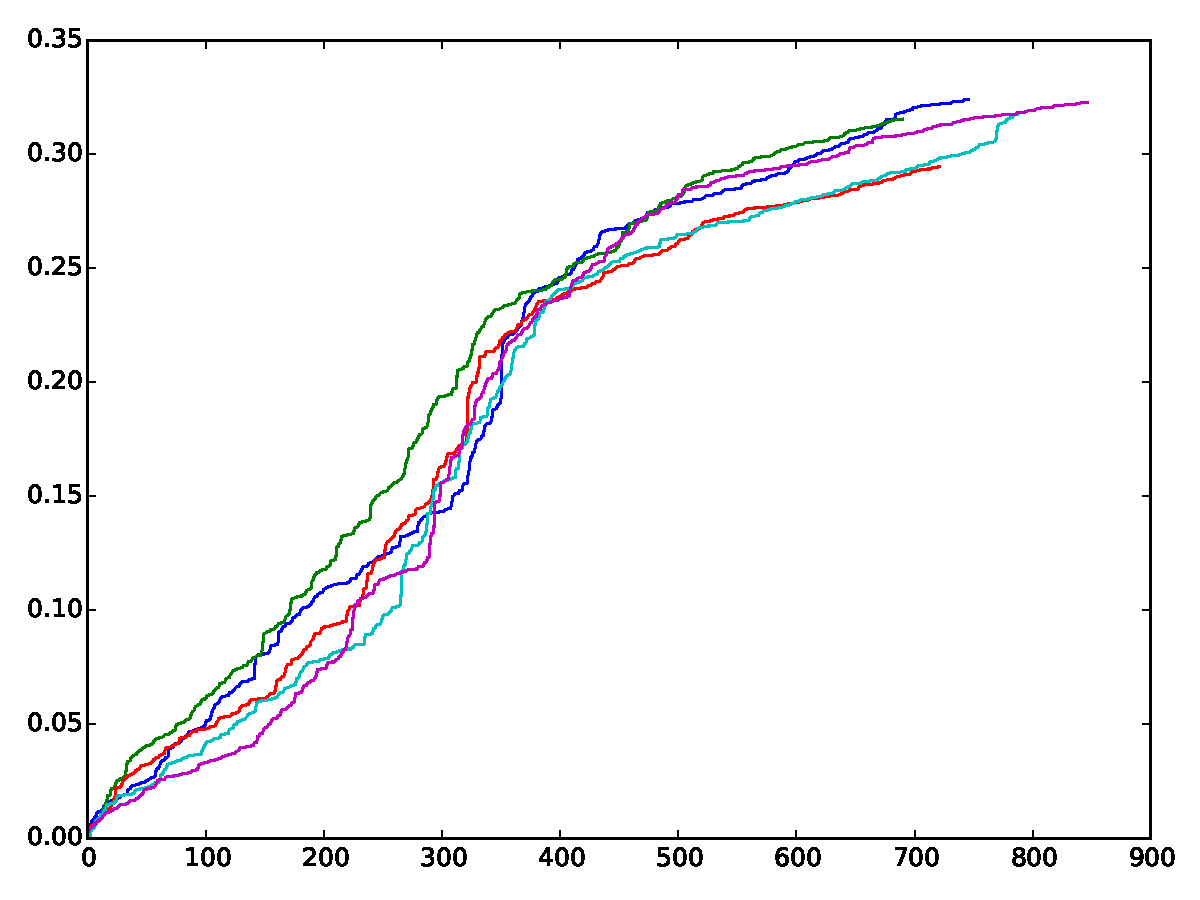
\includegraphics[width=0.7\textwidth]{./figure/smo.pdf}
    \caption{SMO: Dual Objective Value v.s. Number of Iterations}
    \label{fig:smo}
\end{figure}

\problem
\subproblem
\textbf{\em Primal Estimated sub-GrAdient SOlver for SVM (Pegasos)}

The objective function to be optimized is the primal form of Support Vector Machine (SVM):
\begin{equation*}
\min_{w}\frac{\lambda}{2}||w||^2 + \frac{1}{m}\sum_{(x, y) \in S}{l(w; (x, y))}
\end{equation*}
where
\begin{equation*}
l(w; (x, y)) = max\left\{ 0, 1 - y \langle w, x \rangle \right\}
\end{equation*}

The Pegasos algorithm has two parts:
\begin{enumerate}
\item a stochastic gradient descent algorithm
\item a projection over weight vector to the optimal set $B = \left\{ w: ||w|| \leq 1 / \sqrt{\lambda} \right\}$
\end{enumerate}
We will first show why $B$ is the optimal set for $w$ and then give the stochastic gradient descent algorithm based on it.

\textbf{\em Optimal Set for $w$}

In this section we will prove that the optimal $w^*$ must be inside the set $B = \left\{ w: ||w|| \leq 1 / \sqrt{\lambda} \right\}$

\proof
To do so, we examine the dual form of the SVM and use the strong duality theorem. Setting $C = 1 / \lambda m$, the primal objective function can be expressed as the following constrained optimization problem
$$\frac{1}{2}||w||^2 + C\sum_{i = 1}^{m}\xi_{i} ~~ \mathrm{s.t.} ~~ \forall i \in \{1, 2, ... m\}: \xi_{i} \geq 0, ~ \xi_{i} \geq 1 - y_{i} \langle w, x_{i} \rangle $$
Then the Dual or this problem has the form:
$$ \sum_{i = 1}^{m}{\alpha_{i}} - \frac{1}{2}\left|\left|\sum_{i = 1}^{m}{\alpha_{i}y_{i}x_{i}}\right|\right|^2 ~~ \mathrm{s.t.} ~~\forall i \in \{1, 2, ... m\}: 0 \leq \alpha_{i} \leq C$$

Denote the optimal primal and dual solutions by $(w^{*}, \xi^{*})$ and $\alpha^{*}$, respectively. Then the dual objective can be written as
$$||\alpha^{*}||_{1} - \frac{1}{2}||w^{*}||^2$$
By strong duality, the primal objective value is equal to the dual objective value at the optimum, thus
$$\frac{1}{2}||w^{*}||^2 + C||\xi^{*}||_{1} = ||\alpha^{*}||_{1} - \frac{1}{2}||w^{*}||^2$$
Note that $||\alpha^{*}|| \leq C = \frac{1}{\lambda m}$. Therefore, $||\alpha^{*}||_{1} \leq 1 / \lambda$, hence
$$\frac{1}{2}||w^{*}||^2 \leq \frac{1}{2}||w^{*}||^2 + C||\xi^{*}||_{1} = ||\alpha^{*}||_{1} - \frac{1}{2}||w^{*}||^2 \leq \frac{1}{\lambda} - \frac{1}{2}||w^{*}||^2$$
which suggests that
$$||w^*|| \leq \frac{1}{\sqrt\lambda}$$ Q.E.D.

Knowing that the optimal $w^*$ must be inside the set $B = \left\{ w: ||w|| \leq 1 / \sqrt{\lambda} \right\}$, in the stochastic gradient descent we will initialize weight vector $w^{0}$ inside the set $B$, and for each iteration we will project the updated $w^{t}$ to the set $B$. In this way we can accelerate the convergence.
\newline

\textbf{\em Stochastic Gradient Descent Algorithm}

The stochastic gradient descent algorithm is straight forward. For each iteration we randomly pick $k$ observations from the training set as the training subset $A_{t}$, and update weight vector $w$ based on $A_{t}$. Note that when computing the gradient, we only use a subset of $A_{t}$, $A_{t}^{+} = \left\{ i \in A_{t}:~y_{i}\langle w^{t}, x_{i}\rangle < 1   \right\}$, since only observations inside $A_{t}^{+}$ contributes gradient to the hinge loss.
\newline


\textbf{\em The Pegasos Algorithm}

Input: Training set $S$, regularization parameter $\lambda$, number of iterations $T$, size of training subset $k$

Initialize: Choose $w^{0}$ s.t. $||w^{0}|| \leq 1 / \sqrt{\lambda}$

For $t = 0, 1, \dots, T - 1$

\hspace{2ex} Choose $A_{t} \subset S$, where $|A_{t}| = k$

\hspace{2ex} Set $A_{t}^{+} = \left\{ i \in A_{t}:~y_{i}\langle w^{t}, x_{i}\rangle < 1   \right\}$

\hspace{2ex} Set step size $\eta_{t} = \frac{1}{\lambda t}$

\hspace{2ex} Set $w^{t + \frac{1}{2}} = (1 - \eta_{t}\lambda)w^{t} + \frac{\eta_{t}}{k}\sum_{(x,y)\in A_{t}^{+}}{yx}$ \hspace{2ex}(pure gradient descent)

\hspace{2ex} Set $w^{t + 1} = \min\left\{1, \frac{1/\sqrt{\lambda}}{||w^{t + \frac{1}{2}}||}\right\}w^{t + \frac{1}{2}}$ \hspace{2ex}(project $w^{t + \frac{1}{2}}$ into optimal set $B$)

Output: $w^{T}$
\newline

\textbf{\em Simulation Study}

Here we evaluate the optimization performance of Pegasos algorithm by applying it to train SVM model for dataset MNIST-13. We choose $k = 1, 20, 100, 200, 2000$, respectively. For each setting, the model is trained 5 times and the mean and the standard deviation of the training time will be recorded. The result is summarized in table $\ref{sgd}$.

\begin{table}[ht!]
\centering
\caption{Training time for Pegasos algorithm}
\begin{tabular}{rccccc}
\toprule
 \multicolumn{1}{c}{  } & \multicolumn{1}{c}{ $k = 1$ } & \multicolumn{1}{c}{ $k = 20$ } & \multicolumn{1}{c}{ $k = 100$ } & \multicolumn{1}{c}{ $k = 200$ } & \multicolumn{1}{c}{ $k = 2000$ } \\
\midrule
 Avg Time (sec) & $0.228$ & $0.059$ & $0.053$ & $0.056$ & $0.106$ \\
 Std Time (sec) & $0.021$ & $0.004$ & $0.007$ & $0.004$ & $0.007$ \\
\bottomrule
\end{tabular}
\label{sgd}
\end{table}

$***$ Note that the training time for $k = 1$ is unexpected long. This is because when $k$ is too small, it takes time for the algorithm to find an nonempty set $A_{t}^{+}$.

To show the optimization performance, we record the primal objective function for each iteration till convergence and make plots for objective function values over number of iterations in figure \ref{fig:sgd}.

\begin{figure}[ht!]
    \centering
    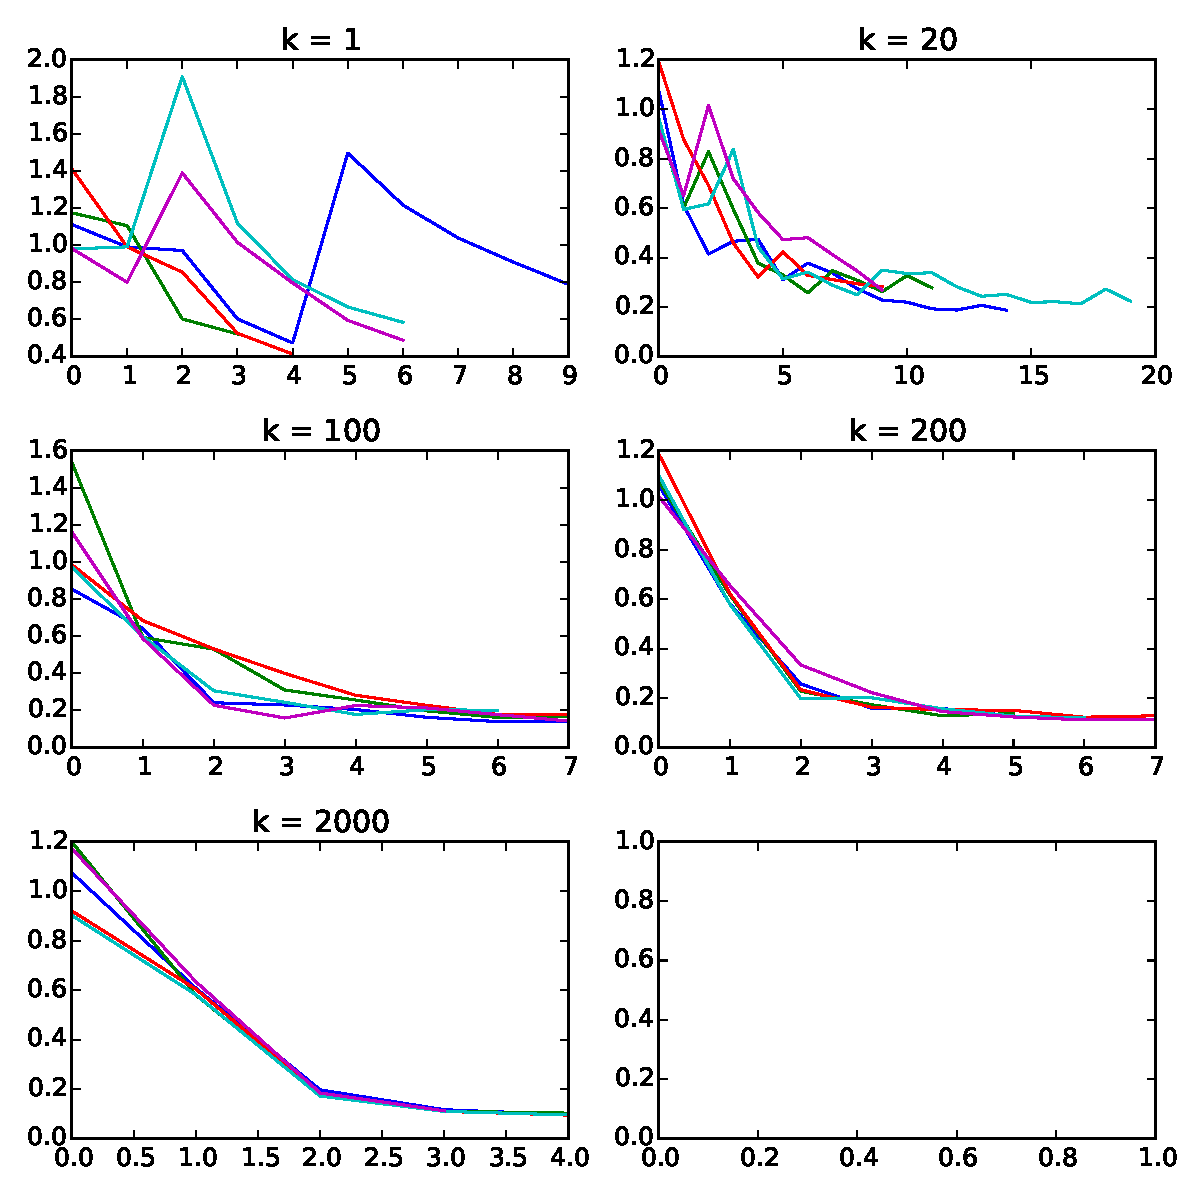
\includegraphics[width=0.9\textwidth]{./figure/sgd.pdf}
    \caption{Pegasos: Primal Objective Value v.s. Number of Iterations}
    \label{fig:sgd}
\end{figure}

\end{document}
